%% Week 44 -- Tuesday session (flipped classroom): cross-validation for the
%% Project 2 network.  SECOND VERSION (2026-10-25): same material as the
%% first, spread over lighter frames.  Precision of 2026-10-25 (evening):
%% REQUIRED in the exercises and in Project 2 is cross-validating the
%% learning rate and the penalty in front of the L2/L1 norm; the width,
%% depth, activation and number of epochs are OPTIONAL there -- the
%% examples (Case 2 step 4) stay so that the students know how.
%% Original header follows: same material as the
%% first, spread over more and lighter frames; Part A is now a 30-minute
%% lecture.  Part A (~30 min): three errors and three data sets, the k-fold
%% estimate and what it estimates (Section 2.12, Eq. 3.92), K from 2 to n,
%% the standard error and why it is optimistic (3.93), the one-standard-
%% error rule (3.96), the refit, leakage and the Pipeline, the
%% hyperparameters of a network and early stopping (Section 8.12),
%% validation curves, the optimism of the best score, what scikit-learn
%% provides and the three rules of an estimator.  Then TWO cases: Case 1 =
%% the six pencil questions of exercise 1 (groups, then plenum with the
%% answers on \pause); Case 2 = the students' own network as a scikit-learn
%% estimator inside KFold, cross_validate, GridSearchCV and
%% validation_curve on the Runge regression of Project 2 (exercise 2).  At
%% the end ONLY a mention of PyTorch and TensorFlow/Keras.  Writing the loop
%% by hand is optional (exercise 4).  First version: _to_delete/
%% week44tuesday_dense.tex.
%% Companion to week44slides.tex (Monday lecture) and to week44tuesday.ipynb.
%% Numbers from make_week44_figures.py, Part 5 (seed 2026, KFold(5,
%% shuffle=True, random_state=2026)), figure week44_cv.pdf; book figure 3.4
%% (cv_ridge_lasso) from BookFigures/chapter03_linear_regression.
%% Build:  pdflatex week44tuesday.tex  (twice)
\documentclass[10pt,aspectratio=169]{beamer}
\usetheme{red_plain}
\usepackage[T1]{fontenc}
\usepackage[utf8]{inputenc}
\usepackage{amsmath,amssymb,bm}
\usepackage{graphicx}
\usepackage{listings}
\usepackage{xcolor}
\usepackage{booktabs}
\graphicspath{{../BookFigures/chapter03_linear_regression/}{./}}

%% ---- code listings
\definecolor{codebg}{rgb}{0.97,0.97,0.97}
\lstset{language=Python,basicstyle=\ttfamily\scriptsize,backgroundcolor=\color{codebg},
  keywordstyle=\color{blue!70!black}\bfseries,commentstyle=\color{green!45!black},
  stringstyle=\color{red!60!black},showstringspaces=false,frame=single,
  framerule=0pt,xleftmargin=4pt,xrightmargin=4pt,breaklines=true,columns=fullflexible}

%% ---- discussion frames (kept for future weeks, unused in this deck)
\newcounter{insight}
\newenvironment{insight}[1][]{%
  \stepcounter{insight}%
  \begin{frame}{Warm-up \arabic{insight}: #1}%
  \setbeamercolor{block title}{bg=structure.fg,fg=white}%
  \setbeamercolor{block body}{bg=structure.fg!8}%
}{\end{frame}}
\newcommand{\question}[1]{\begin{block}{Question}#1\end{block}}
\newcommand{\answer}[1]{\pause\begin{block}{Answer}#1\end{block}}

%% ---- case frames
\newcounter{case}
\newenvironment{case}[1][]{%
  \stepcounter{case}%
  \begin{frame}[fragile,environment=case]{Case \arabic{case}: #1}%
}{\end{frame}}

\setbeamertemplate{footline}[frame number]
\setbeamertemplate{blocks}[rounded][shadow=false]
\setbeamerfont{block title}{size=\small}
\setbeamercovered{invisible}

\title{Week 44, Tuesday Session}
\subtitle{Flipped classroom: cross-validation for your Project 2 network --
  half an hour of theory, then the six questions of exercise 1, then your
  own network inside \texttt{scikit-learn}\\[3pt]
  \small Companion notebook: \texttt{week44tuesday.ipynb}}
\author{Morten Hjorth-Jensen}
\institute{Department of Physics and Center for Computing in Science Education,\\
  University of Oslo, Norway}
\date{}

\begin{document}

\begin{frame}
\titlepage
\end{frame}

\begin{frame}{How today works}
\small
\begin{block}{Part A (about 30 minutes, a regular lecture)}
The theory of cross-validation in one pass: three errors and three data
sets; the $k$-fold estimate, its standard error and the one-standard-error
rule; leakage and why the scaler lives inside the fold; the hyperparameters
of a network, epochs among them; what \texttt{scikit-learn} provides.
\end{block}
\begin{block}{Case 1 (about 20 minutes): the six questions}
Exercise 1 of \texttt{exercisesweek44.ipynb}, in groups, pencil and paper;
then the answers in plenum, one at a time.
\end{block}
\begin{block}{Case 2 (about 35 minutes): your network inside \texttt{scikit-learn}}
Exercise 2: wrap your own network as an estimator, then let \texttt{KFold},
\texttt{cross\_validate}, \texttt{GridSearchCV} and
\texttt{validation\_curve} do the folds, the scaling inside the folds, the
grid and the bookkeeping.  Six steps, checkpoints after each; step 4
(width, epochs) is the optional part.
\end{block}
\begin{block}{Last five minutes}
What to finish before Friday; a mention -- only a mention -- of how the
same is done with PyTorch and Keras; what next Monday builds on.
\end{block}
\end{frame}

\begin{frame}{What you need, and what today is for}
\small
\begin{block}{What you need}
Your Project 2 network (or the week-41 code: \texttt{create\_layers},
\texttt{train}, \texttt{predict}), \texttt{scikit-learn}, and the data cell
of Project 2 part b) -- $100$ points of the Runge function with noise
$\sigma=0.1$, seed $2026$.  The notebook has everything, with the week-41
network filled in as the estimator.
\end{block}
\begin{block}{What today is for -- and what is required}
Every number you report on the test set must come from a model whose every
choice was made on training data alone -- today is how.  \textbf{Required},
in exercise 2 and in Project 2: cross-validate the learning rate $\gamma$
and the penalty $\lambda$ in front of the L2 or L1 norm (the heat map of
Case 2, step 3).
\end{block}
\begin{block}{What is optional}
Cross-validating the width, the depth, the activation and the number of
epochs (Case 2, step 4; exercise 2 c--d) -- optional in the exercises and in
Project 2, shown today so that you know how; the machinery is the same.
Writing the cross-validation loop yourself (exercise 4).  Understanding
what the library does is not optional.
\end{block}
\end{frame}

%% =====================================================================
\section{Part A: the theory}
\begin{frame}{Part A.1: two kinds of unknowns}
\small
\begin{block}{Parameters}
The weights and biases of the network (or $\bm{\theta}$ of a linear
model).  For given hyperparameters they are fixed by \emph{minimising the
cost on the training data}.
\end{block}
\begin{block}{Hyperparameters}
The penalty $\lambda$, the learning rate $\gamma$, the width and depth,
the activation, the batch size, the number of epochs.  They cannot be
fixed by the same minimisation, and the reason is exact.
\end{block}
\begin{block}{Why the training error cannot choose them (3.91)}
The training error is non-decreasing in $\lambda$ along the whole path,
\[
  \mathrm{Err}_{\mathrm{Train}}(\lambda)\ \ge\ \mathrm{Err}_{\mathrm{Train}}(0),
\]
so minimising it over $\lambda$ always returns $\lambda=0$.  It
\emph{falls} with every hidden unit and every epoch, so minimising it over
those returns the widest network trained longest.  The training error
chooses nothing.
\end{block}
\end{frame}

\begin{frame}{Part A.2: three errors, three data sets}
\small
\begin{columns}[T]
\begin{column}{0.5\textwidth}
\begin{block}{Three errors, kept apart}
\begin{enumerate}
  \item the \textbf{training error}: minimised over the parameters, at
        fixed hyperparameters;
  \item the \textbf{cross-validation error}: minimised over the
        hyperparameters;
  \item the \textbf{test error}: computed \emph{once}, at the very end,
        minimised over nothing.
\end{enumerate}
\end{block}
\end{column}
\begin{column}{0.48\textwidth}
\begin{block}{Three data sets}
\begin{itemize}
  \item the \textbf{test set}: set aside first, not looked at until the
        last step;
  \item the \textbf{training data}: everything else -- scaling, folds,
        grid and refit all happen inside it;
  \item the \textbf{validation fold}: a piece of the training data that
        plays the test set's role while choices are made.
\end{itemize}
\end{block}
\end{column}
\end{columns}
\medskip
$k$-fold cross-validation lets every training point play the validation
role exactly once.  That is the whole idea; the rest of Part A is the
details that make it correct.
\end{frame}

\begin{frame}{Part A.3: the recipe of Section 3.14, which Case 2 follows}
\small
\begin{enumerate}
  \item Set aside a test set and do not look at it again until step 6.
  \item Choose a grid of hyperparameter values -- logarithmic for $\gamma$
        and $\lambda$.
  \item Shuffle the training data and split it into $K$ folds, $K$ between
        five and ten.
  \item For every fold and every grid point: standardise with the
        \emph{training folds'} statistics, fit on the training folds,
        predict the held-out fold, record the error.  Average to obtain
        the CV error and its standard error.
  \item Select the minimum, or the one-standard-error choice, and
        \emph{refit on all the training data} at that value.
  \item Evaluate the refitted model on the test set, once.  Report the
        selected hyperparameters, the CV error with its standard error,
        and the test error.
\end{enumerate}
\medskip
Six steps, six places where something can go wrong.  Part A takes them in
turn.
\end{frame}

\begin{frame}{Part A.4: the $k$-fold estimate (Section 2.12, Eq.~3.92)}
\small
Shuffle; cut into $K$ folds of equal size; let $\kappa(i)$ be the fold of
observation $i$.  For each fold $k$: hold it out, fit on the other $K-1$,
predict the held-out fold, discard the model.
\begin{block}{The cross-validation error}
The average error of every observation predicted by the model that
\emph{did not see it}:
\[
  \mathrm{CV}_K=\frac{1}{n}\sum_{i=0}^{n-1}\bigl(y_i-\hat f^{(-\kappa(i))}(\bm{x}_i)\bigr)^{2}
  =\frac{1}{K}\sum_{k=1}^{K}\mathrm{MSE}_k .
\]
\end{block}
Every observation is validated exactly once and trained on $K-1$ times.
The $K$ fold models are temporary: averaged, then thrown away.
\end{frame}

\begin{frame}{Part A.5: what the estimate is \emph{of} -- read this twice}
\small
\begin{block}{The statement}
$\mathrm{CV}_K$ estimates the expected error on unseen data of the
\textbf{training procedure} -- this architecture, these hyperparameters,
this optimiser -- applied to \emph{training sets of size $n(K-1)/K$}.
\end{block}
\begin{block}{What it is not}
Not the error of the one network you finally train on all $n$ points.
That network is a \emph{new} fit, which cross-validation never evaluated.
\end{block}
\begin{block}{Why the estimate is still the right one to use}
The final model is the same recipe applied to slightly more data, so the
CV error is the best available estimate of its error -- slightly
pessimistic, because the fold models had $n/K$ fewer points.
\end{block}
\end{frame}

\begin{frame}{Part A.6: choosing $K$, from $2$ to $n$}
\small
\begin{columns}[T]
\begin{column}{0.5\textwidth}
\begin{block}{Small $K$}
The fold models train on much less than $n$ points: the estimate is
\emph{biased upwards} (pessimistic).  For $K=2$ the procedure is judged on
half the data.
\end{block}
\begin{block}{$K=n$, leave-one-out}
No bias from the training-set size and no randomness from the fold
assignment -- it is the jackknife of Eq.~(2.53) applied to prediction.
But $n$ fits, and the $n$ training sets are almost identical, so the fold
errors are strongly correlated and the estimate has \emph{high
variance}.
\end{block}
\end{column}
\begin{column}{0.48\textwidth}
\begin{block}{The compromise}
$K=5$ or $K=10$.
\end{block}
\begin{block}{What it costs for a network}
$K$ folds $\times$ every grid point $\times$ every epoch.  Case 2 has
$5\times25\times1000$ epochs on $80$ points -- a minute.  On MNIST,
exercise 3 prescribes a $10\,000$-image subset for a reason, and random
search over the grid (Section 8.12) is often the better use of the budget.
\end{block}
\begin{block}{Classification}
Cut \emph{within each class}, so that every fold carries the class
proportions -- \texttt{StratifiedKFold}.  Otherwise a rare class may be
missing from a training fold entirely.
\end{block}
\end{column}
\end{columns}
\end{frame}

\begin{frame}{Part A.7: the standard error, and why it is optimistic (Eq.~3.93)}
\small
\begin{block}{The spread of the $K$ fold errors}
\[
  \mathrm{SE}_K=\frac{1}{\sqrt K}\sqrt{\frac{1}{K-1}\sum_{k=1}^{K}
  \bigl(\mathrm{MSE}_k-\mathrm{CV}_K\bigr)^{2}}
  \qquad\text{-- Eq.~(2.24) applied to $K$ numbers.}
\]
\end{block}
\begin{block}{A rough guide, not a confidence interval}
Two training sets of a $K$-fold share a fraction $(K-2)/(K-1)$ of their
points -- $3/4$ for $K=5$.  The fold errors are therefore positively
correlated, and (3.93) \emph{understates} the true uncertainty.
\end{block}
\begin{block}{A library detail that bites}
\texttt{GridSearchCV} reports \texttt{std\_test\_score} with
\texttt{ddof=0}.  The standard error of (3.93) is
\texttt{std\_test\_score / np.sqrt(K - 1)}.  And every score is a
\emph{negative} MSE, because the library maximises.
\end{block}
\end{frame}

\begin{frame}{Part A.8: the one-standard-error rule (Eq.~3.96)}
\small
\begin{block}{The problem}
Near its minimum the CV curve is flat, and the position of the minimum is
known only to within the noise of the estimate.
\end{block}
\begin{block}{The rule}
Among the hyperparameters whose CV errors are within one standard error
of the best, take the \emph{simplest}:
\[
  \lambda_{1\mathrm{SE}}=\max\bigl\{\lambda:\ \mathrm{CV}_K(\lambda)\le
  \mathrm{CV}_K(\lambda_{\min})+\mathrm{SE}_K(\lambda_{\min})\bigr\}.
\]
The improvement offered by the more complex model is not larger than the
uncertainty with which it is measured, so it is not believed.  A
convention, not a theorem -- and it errs deliberately towards simplicity.
\end{block}
\begin{block}{``Simplest'' for a network}
Largest $\lambda$; \emph{fewest} hidden units; \emph{fewest} epochs.  The
learning rate affects the optimiser, not the model, so on a two-axis grid
apply the rule along the regularisation axis.
\end{block}
\end{frame}

\begin{frame}{Part A.9: book Figure 3.4, from week 36 -- the picture does not change}
\begin{center}
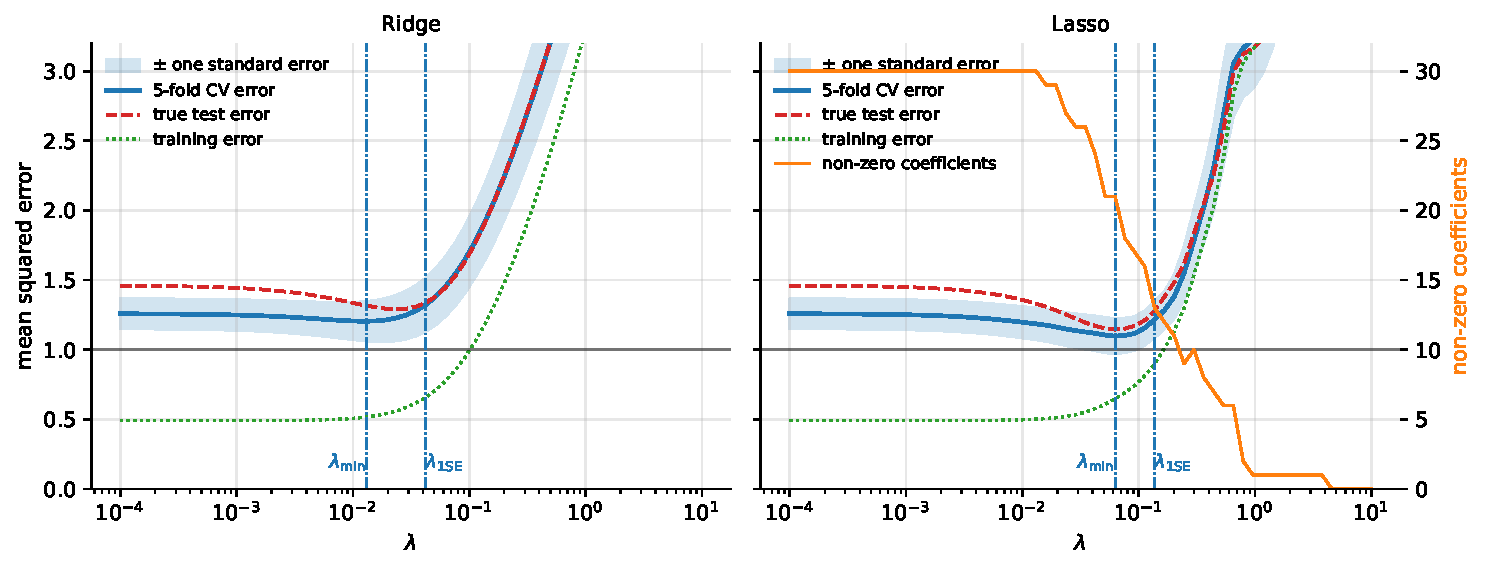
\includegraphics[width=0.72\textwidth]{cv_ridge_lasso}
\end{center}
\small
The CV curve with its standard errors, the minimum, the one-SE choice,
and (dashed) the true test error of the refit, for Ridge and the Lasso on
a sparse truth.  Today the model is a neural network and the axis may be
the learning rate, the width or the number of epochs; the picture, and the
way to read it, are the same.
\end{frame}

\begin{frame}{Part A.10: then refit}
\small
\begin{block}{The final model}
A \emph{new} fit at the chosen hyperparameters on all $n$ training points,
scaled with the statistics of all $n$.  In \texttt{scikit-learn}:
\texttt{best\_estimator\_}, produced by \texttt{refit=True}, the default
of \texttt{GridSearchCV}.
\end{block}
\begin{block}{Which $\lambda$ is being transferred (3.95)}
The fold models were fitted to $n(K-1)/K$ points, the final model to $n$.
With the cost written \emph{per observation},
$\tfrac1n\|\bm{y}-\bm{X}\bm{\theta}\|^{2}+\lambda\|\bm{\theta}\|^{2}$ --
the convention of Project 2 and of our network -- a $\lambda$ found on
$80$ points is the right $\lambda$ for $100$.
\end{block}
\begin{block}{Only then}
The test set, once.
\end{block}
\end{frame}

\begin{frame}{Part A.11: leakage -- the held-out fold is future data}
\small
\begin{block}{The rule}
Nothing computed from the held-out fold may enter the fit.  Any
preprocessing that \emph{learns} from the data -- centring, scaling,
feature selection, imputation, PCA -- is fitted inside each fold, on the
training part only, and applied frozen to the held-out part.
\end{block}
\begin{block}{What leaks if you scale first}
Standardise the whole training set once, and every training fold has seen
the \emph{mean and variance of its own validation fold}.  For scaling
alone the leak is small.  For anything that looks at the targets it is
large: screen the features by their correlation with $y$ on the whole
set, cross-validate the survivors, and the CV error can fall below the
noise floor for features that are pure noise (Section 3.14).
\end{block}
\begin{block}{For a network}
The same for the inputs; and the early-stopping epoch (next frame) must be
chosen on a validation fold, never on the fold being scored.
\end{block}
\end{frame}

\begin{frame}{Part A.12: the mechanism -- a \texttt{Pipeline}}
\small
\begin{center}
\large\texttt{net = make\_pipeline(StandardScaler(), YourNet())}
\end{center}
\begin{itemize}
  \item Cross-validate the \emph{pipeline}, not the network.
  \item On every fold the library calls \texttt{fit} on the pipeline: it
        fits the scaler on the training part, transforms it, fits the
        network on the result.
  \item At prediction time it transforms the held-out part with the
        \emph{stored} training statistics.
  \item Hyperparameters are addressed through the step name:
        \texttt{yournet\_\_gamma}, \texttt{yournet\_\_lmbd} (two
        underscores; the step name is the class name in lower case;
        \texttt{net.get\_params().keys()} lists them all).
\end{itemize}
\medskip
Nothing else enforces the rule of the previous frame.  The pipeline is
how you make leakage impossible rather than merely avoided.
\end{frame}

\begin{frame}{Part A.13: the hyperparameters of a network (Section 8.12)}
\small
\begin{block}{The list}
Learning rate $\gamma$ and the optimiser's own knobs; penalty $\lambda$
(L2, L1); width and depth; activation; batch size; \textbf{number of
epochs}; initialisation seed; dropout rate.
\end{block}
\begin{block}{Two facts about all of them, and what we ask of you}
None can be chosen by the training error.  All of them change the test
error, and strongly: in Case 2 the CV error moves by a factor of four
across the $\gamma$ grid alone.  Required in exercise 2 and Project 2:
$\gamma$ and $\lambda$.  Optional: width, depth, activation, epochs -- same
tools, your choice.
\end{block}
\begin{block}{Epochs are a hyperparameter: early stopping}
The training error falls with every epoch and says nothing.  The
validation error falls, flattens and -- for a network that can overfit --
rises again; the epoch at which it is smallest is the chosen number of
epochs.  Two ways with the library: a \texttt{validation\_curve} over
\texttt{epochs} (Case 2, step 4; a full training per value), or an
estimator that records the validation error \emph{during} one training
run and keeps the best weights (what Keras' \texttt{EarlyStopping} does;
exercise 2d invites you to build one).
\end{block}
\end{frame}

\begin{frame}{Part A.14: validation curves, and the optimism of the best score}
\small
\begin{block}{Validation curves}
One hyperparameter at a time, the others fixed: CV error and training
error against the value, with the standard error.  Where the two curves
separate the model begins to overfit; where the CV curve is flat the data
cannot tell the values apart.  The figures parts c)--d) of Project 2 ask
for are exactly these.
\end{block}
\begin{block}{The best CV score of a grid is optimistic}
The minimum of $25$ noisy estimates is biased \emph{downwards}: you chose
it because it was low, and part of why it was low is noise.  The CV error
of the winner is therefore \emph{not} an unbiased estimate of its test
error.  That is what the test set, touched once at the end, is for -- or
nested cross-validation, an outer loop around the whole selection, when
there is no test set to spare.
\end{block}
\begin{block}{Reporting}
The chosen hyperparameters and how they were chosen; the CV error $\pm$
standard error \emph{and} the training error beside it; the test error,
once.  ``The best learning rate is $0.01$, test MSE $0.0094$'' reports a
choice made on the test set -- Case 1, question d).
\end{block}
\end{frame}

\begin{frame}{Part A.15: what \texttt{scikit-learn} provides}
\small
\begin{center}
\begin{tabular}{@{}ll@{}}
\toprule
theory & library\\
\midrule
the folds & \texttt{KFold(k, shuffle=True, random\_state)}\\
stratified folds & \texttt{StratifiedKFold}\\
the $K$ fold errors, (3.92) & \texttt{cross\_val\_score}\\
plus training errors and fit times & \texttt{cross\_validate}\\
the grid, (3.94), and the refit & \texttt{GridSearchCV}, \texttt{best\_estimator\_}\\
every number of the grid & \texttt{cv\_results\_}\\
one hyperparameter at a time & \texttt{validation\_curve}\\
error against training-set size & \texttt{learning\_curve}\\
out-of-fold predictions & \texttt{cross\_val\_predict}\\
scaling inside the fold & \texttt{Pipeline}\\
\bottomrule
\end{tabular}
\end{center}
\medskip
What they do \emph{not} do: choose the grid, apply the one-standard-error
rule (\texttt{cv\_results\_} has what you need), or stop you from calling
\texttt{fit} on the test set.
\end{frame}

\begin{frame}[fragile]{Part A.16: the three rules of an estimator -- all the library asks of your code}
\small
\begin{columns}[T]
\begin{column}{0.46\textwidth}
\begin{enumerate}
  \item \texttt{\_\_init\_\_} stores its keyword arguments \emph{under the
        same names} and does nothing else.  \texttt{BaseEstimator} then
        supplies \texttt{get\_params}/\texttt{set\_params} -- how
        \texttt{GridSearchCV} sets $\gamma$ and $\lambda$ -- and
        \texttt{clone} gives every fold a fresh, untrained copy.
  \item \texttt{fit(X, y)} does all the work, stores the result in
        attributes ending in an underscore (\texttt{self.layers\_}), and
        \emph{returns \texttt{self}}.
  \item \texttt{predict(X)} returns a 1D array; \texttt{RegressorMixin}
        supplies \texttt{score} (the $R^{2}$).  A classifier adds
        \texttt{predict\_proba} and \texttt{classes\_}.
\end{enumerate}
\end{column}
\begin{column}{0.52\textwidth}
\begin{lstlisting}
class NeuralNetRegressor(BaseEstimator, RegressorMixin):
    def __init__(self, hidden=(50,), activation="sigmoid",
                 gamma=0.03, lmbd=0.0, epochs=1000,
                 batch_size=10, seed=2026):
        self.hidden = hidden
        self.activation = activation
        self.gamma = gamma
        self.lmbd = lmbd
        self.epochs = epochs
        self.batch_size = batch_size
        self.seed = seed

    def fit(self, X, y):
        ...          # your training code; store self.layers_
        return self

    def predict(self, X):
        ...          # your forward pass, shape (len(X),)
\end{lstlisting}
\end{column}
\end{columns}
\end{frame}

%% =====================================================================
\section{Case 1}
\begin{case}[the six questions of exercise 1 -- pencil and paper, in groups]
\small
\begin{block}{a) What is estimated}
In one sentence: the $k$-fold CV error estimates the error of \emph{which}
model, trained on how much data, evaluated on what?  Why is it about the
training \emph{procedure} rather than the one network you train at the end?
\end{block}
\begin{block}{b) The mean and its error}
Give $\bar e\pm s/\sqrt k$ for the $k$ fold errors.  Why are the $k$
numbers not independent (what fraction do two training sets share?), and
what does that do to the standard error?  Bias and variance of the
estimate as $k$ goes from $2$ to $n$?
\end{block}
\begin{block}{c) Scaling}
Why must the scaler be fitted \emph{inside} each fold?  Name one number
that leaks otherwise.  How does a \texttt{Pipeline} guarantee it, in one
sentence?
\end{block}
\end{case}

\begin{frame}{Case 1: the six questions, continued}
\small
\begin{block}{d) The colleague}
``Ten networks, ten learning rates, the test MSE of each; the best learning
rate is $0.01$, with a test MSE of $0.0094$.''  Two things are wrong.
Write the honest version.
\end{block}
\begin{block}{e) Early stopping}
Why is the number of epochs a hyperparameter like any other?  How is a
validation fold used to choose it, and why is the training error useless
for that?
\end{block}
\begin{block}{f) The one-standard-error rule}
State it for $\lambda\in\{0,10^{-5},\dots,10^{-2}\}$.  Why does it prefer
the \emph{more} regularised model among those within one standard error --
and what does ``more regularised'' mean when the grid is over hidden
units?
\end{block}
\begin{block}{Procedure}
Fifteen minutes in your group, write the answers in the notebook; then
plenum, one question at a time.  Nothing is computed in Case 1.
\end{block}
\end{frame}

\begin{frame}{Case 1: what we hope you say (a--b)}
\small
\setbeamercolor{block title}{bg=structure.fg,fg=white}
\setbeamercolor{block body}{bg=structure.fg!8}
\pause
\begin{block}{a)}
The expected error, on data drawn from the same distribution and never
seen in training, of the \emph{procedure} ``this architecture with these
hyperparameters, trained this way on $n(k-1)/k$ points'' -- averaged over
which points those are.  It is about the procedure because the $k$ fold
models are different networks (different training sets, same recipe) that
are averaged and discarded; the network you keep is a new fit on all $n$
points, which CV never evaluated.
\end{block}
\pause
\begin{block}{b)}
$\bar e=\frac1k\sum e_j$, $s^{2}=\frac{1}{k-1}\sum(e_j-\bar e)^{2}$,
standard error $s/\sqrt k$ (3.93).  Two training sets each omit one fold
and share the other $k-2$ of the $k-1$ folds they contain: a fraction
$(k-2)/(k-1)$ in common, $3/4$ for $k=5$.  Positively correlated fold
errors have a larger variance of the mean than independent ones, so
$s/\sqrt k$ is \emph{optimistic}.  $k=2$: training sets of $n/2$, a
pessimistic estimate but nearly independent folds; $k=n$: no size bias
and no fold randomness, but $n$ almost identical training sets, highly
correlated errors, high variance, and $n$ fits.
\end{block}
\end{frame}

\begin{frame}{Case 1: what we hope you say (c--d)}
\small
\setbeamercolor{block title}{bg=structure.fg,fg=white}
\setbeamercolor{block body}{bg=structure.fg!8}
\pause
\begin{block}{c)}
Fitted on all the data, the scaler has seen the mean and the standard
deviation of the held-out fold, so information about the validation points
enters the training -- the held-out fold is no longer ``future data''.  The
numbers that leak: the fold's mean and variance of $x$ (and of $y$ if the
targets are scaled).  A \texttt{Pipeline} refits \emph{every} step on the
training part of each fold when the library calls \texttt{fit}, and uses
the stored statistics when it calls \texttt{predict} on the held-out part.
\end{block}
\pause
\begin{block}{d)}
First, the learning rate was \emph{chosen on the test set}: the test MSE
was minimised over ten candidates, so $0.0094$ is the minimum of ten noisy
numbers and no longer estimates the error of anything.  Second, there is
no uncertainty: ten single numbers, no standard error.  Honest version:
``Of ten learning rates, five-fold cross-validation on the training data
selected $\gamma=0.01$ with a CV MSE of $x\pm s$ (training MSE $y$); the
network refitted at $\gamma=0.01$ on all training data has a test MSE of
$z$, computed once.''
\end{block}
\end{frame}

\begin{frame}{Case 1: what we hope you say (e--f)}
\small
\setbeamercolor{block title}{bg=structure.fg,fg=white}
\setbeamercolor{block body}{bg=structure.fg!8}
\pause
\begin{block}{e)}
The number of epochs changes the fitted function exactly as $\lambda$ or
the width does -- a network trained for $100$ epochs and one trained for
$3000$ are different models -- and it cannot be chosen by the training
error, which is non-increasing in the epochs by construction.  Hold out a
validation fold, record its error after every epoch, take the epoch at
which it is smallest, and train the final model for that many epochs (or
keep the weights of that epoch).  Averaged over folds this is a validation
curve over epochs.
\end{block}
\pause
\begin{block}{f)}
$\lambda_{1\mathrm{SE}}=\max\{\lambda:\mathrm{CV}(\lambda)\le
\mathrm{CV}(\lambda_{\min})+\mathrm{SE}(\lambda_{\min})\}$: the largest
penalty whose CV error is within one standard error of the best.  The
models in that set cannot be told apart by the data, so the improvement of
the less regularised one is not believed, and the simpler model has lower
variance.  Over hidden units ``more regularised'' means \emph{fewer} units
-- the smallest network within one standard error of the best; over
epochs, the fewest epochs.
\end{block}
\end{frame}

%% =====================================================================
\section{Case 2}
\begin{case}[your network inside \texttt{scikit-learn}'s cross-validation]
\small
\begin{block}{The data and the folds}
The data cell of Project 2 part b), verbatim: $n=100$, $x$ uniform on
$[-1,1]$, $y=1/(1+25x^{2})+\varepsilon$, $\sigma=0.1$, seed $2026$.  One
\texttt{KFold(5, shuffle=True, random\_state=2026)} object, used for
\emph{everything} below so that every comparison is on the same folds.
\end{block}
\begin{block}{Step 1: the wrapper}
Fill in \texttt{fit} and \texttt{predict} around your network (the three
rules of Part A.16).  \emph{Checkpoint:} \texttt{fit} on all $100$ points,
\texttt{predict} on them, and the training MSE agrees with your own loop to
every digit.
\end{block}
\begin{block}{Step 2: a first look}
\texttt{cross\_val\_score} on the pipeline \texttt{StandardScaler $\to$
net}: five negative MSEs; mean $\pm$ $s/\sqrt5$.
\texttt{cross\_validate} for the training MSEs beside them.
\emph{Checkpoint:} the training MSE is below the CV MSE, both above
$\sigma^{2}=0.01$.
\end{block}
\begin{block}{Step 3: the grid}
\texttt{GridSearchCV} over
$\gamma\in\{0.001,\dots,0.1\}\times\lambda\in\{0,10^{-5},\dots,10^{-2}\}$;
from \texttt{cv\_results\_}: heat map, standard errors
(\texttt{std\_test\_score}$/\sqrt{k-1}$), the one-standard-error choice.
\end{block}
\end{case}

\begin{frame}{Case 2: steps 4--6}
\small
\begin{block}{Step 4 (optional): validation curves}
\texttt{validation\_curve} over the hidden units $\{5,10,25,50,100\}$ and
over the epochs $\{50,\dots,3000\}$: CV and training MSE against the
value.  \emph{Checkpoint:} the training curve only falls -- where does the
CV curve stop falling?  Optional in exercise 2 and Project 2; same
machinery as step 3.
\end{block}
\begin{block}{Step 5: the benchmark}
OLS and Ridge polynomials of degree $1$--$15$ on the \emph{same}
\texttt{cv}: one table with CV MSE $\pm$ s.e., parameters and
\texttt{mean\_fit\_time} for the polynomial and the network.
\end{block}
\begin{block}{Step 6: the test set, once}
A fresh set of $100$ points (seed $1$); \texttt{best\_estimator\_} -- the
winner refit on all $100$ training points -- is evaluated on it once, and
so is the polynomial.  No going back.
\end{block}
\begin{block}{Numbers to write down}
The five fold errors; the best grid point with its error bar and the
one-SE choice; the test MSE of network and polynomial -- these go into
Project 2.  If you did step 4: where the CV curves stop falling.  Each
fit takes under a second, the grid about a minute.
\end{block}
\end{frame}

\begin{frame}[fragile]{Case 2: the code you should end up with (steps 1--2)}
\lstset{basicstyle=\ttfamily\fontsize{7}{7.6}\selectfont}
\begin{columns}[T]
\begin{column}{0.66\textwidth}
\begin{lstlisting}
class Week41Regressor(BaseEstimator, RegressorMixin):
    def __init__(self, ...):    # as on the Part A.16 frame
        ...
    def fit(self, X, y):
        rng = np.random.default_rng(self.seed)
        sizes = [X.shape[1], *self.hidden, 1]
        layers = create_layers(sizes, self.activation, rng)
        self.layers_, self.history_ = train(
            X, y.reshape(-1, 1), layers, self.activation,
            "mse", gamma=self.gamma, epochs=self.epochs,
            batch_size=self.batch_size, lmbd2=self.lmbd,
            rng=rng)
        return self
    def predict(self, X):
        out = predict(X, self.layers_, self.activation, "mse")
        return out[:, 0]

cv = KFold(n_splits=5, shuffle=True, random_state=2026)
net = make_pipeline(StandardScaler(), Week41Regressor())
mse = "neg_mean_squared_error"
scores = -cross_val_score(net, X, y, cv=cv, scoring=mse)
print(scores.mean(), scores.std(ddof=1) / np.sqrt(5))
res = cross_validate(net, X, y, cv=cv, scoring=mse,
                     return_train_score=True)
\end{lstlisting}
\end{column}
\begin{column}{0.32\textwidth}
\small
\begin{itemize}
  \item \texttt{fit} builds the layers from the seed and calls the
        week-41 \texttt{train}; \texttt{predict} runs the forward pass and
        flattens to 1D.
  \item \texttt{y.reshape(-1, 1)}: the week-41 code wants a column; the
        library hands over a 1D array.
  \item Every fold starts from \texttt{clone(net)}: a fresh scaler and a
        fresh, untrained network with the same seed.
  \item \texttt{scores} are negative MSEs: flip the sign.
\end{itemize}
\end{column}
\end{columns}
\end{frame}

\begin{frame}[fragile]{Case 2: the code you should end up with (steps 3--4)}
\begin{columns}[T]
\begin{column}{0.66\textwidth}
\begin{lstlisting}
grid = {"week41regressor__gamma":
            [0.001, 0.003, 0.01, 0.03, 0.1],
        "week41regressor__lmbd":
            [0.0, 1e-5, 1e-4, 1e-3, 1e-2]}
search = GridSearchCV(net, grid, cv=cv, scoring=mse,
                      return_train_score=True).fit(X, y)
r = search.cv_results_
cvmse = -r["mean_test_score"].reshape(5, 5)
se = r["std_test_score"].reshape(5, 5) / np.sqrt(5 - 1)
best = search.best_index_                        # ddof=0 !
within = cvmse <= cvmse.min() + se.ravel()[best]

tr, va = validation_curve(
    net, X, y, cv=cv, scoring=mse,
    param_name="week41regressor__hidden",
    param_range=[(5,), (10,), (25,), (50,), (100,)])
# tr, va: (5 values, 5 folds); the same for "...__epochs\"
\end{lstlisting}
\end{column}
\begin{column}{0.32\textwidth}
\small
\begin{itemize}
  \item \texttt{week41regressor\_\_gamma}: step name, two underscores,
        parameter name.
  \item \texttt{cv\_results\_} is a dictionary of arrays, one entry per
        grid point, in the order of \texttt{params}; reshape to the grid.
  \item \texttt{std\_test\_score} is the population standard deviation
        (\texttt{ddof=0}), hence the $\sqrt{k-1}$.
  \item \texttt{validation\_curve} is one-dimensional grid search that
        hands back the training scores too.
\end{itemize}
\end{column}
\end{columns}
\end{frame}

\begin{frame}[fragile]{Case 2: the code you should end up with (steps 5--6)}
\begin{columns}[T]
\begin{column}{0.66\textwidth}
\begin{lstlisting}
poly = make_pipeline(StandardScaler(), PolynomialFeatures(),
                     LinearRegression())
ols = GridSearchCV(poly,
        {"polynomialfeatures__degree": range(1, 16)},
        cv=cv, scoring=mse).fit(X, y)
# the same with Ridge(alpha=...) for LinearRegression()

X_test, y_test = fresh_data(seed=1)      # once, at the end
pred = search.best_estimator_.predict(X_test)
mse_test = np.mean((pred - y_test) ** 2)
pred = ols.best_estimator_.predict(X_test)
mse_ols = np.mean((pred - y_test) ** 2)
\end{lstlisting}
\end{column}
\begin{column}{0.32\textwidth}
\small
\begin{itemize}
  \item The polynomial runs on the \emph{same} \texttt{cv}: that is what
        makes the comparison fair.
  \item \texttt{best\_estimator\_} is the whole pipeline -- scaler and
        network -- refit on all $100$ points.
  \item The test set is generated (or unpacked) here and nowhere earlier;
        it is used once, for every model, and nothing is changed afterwards.
\end{itemize}
\end{column}
\end{columns}
\end{frame}

\begin{frame}{Case 2: what you should find (\texttt{week44\_cv.pdf}, seed 2026)}
\begin{center}
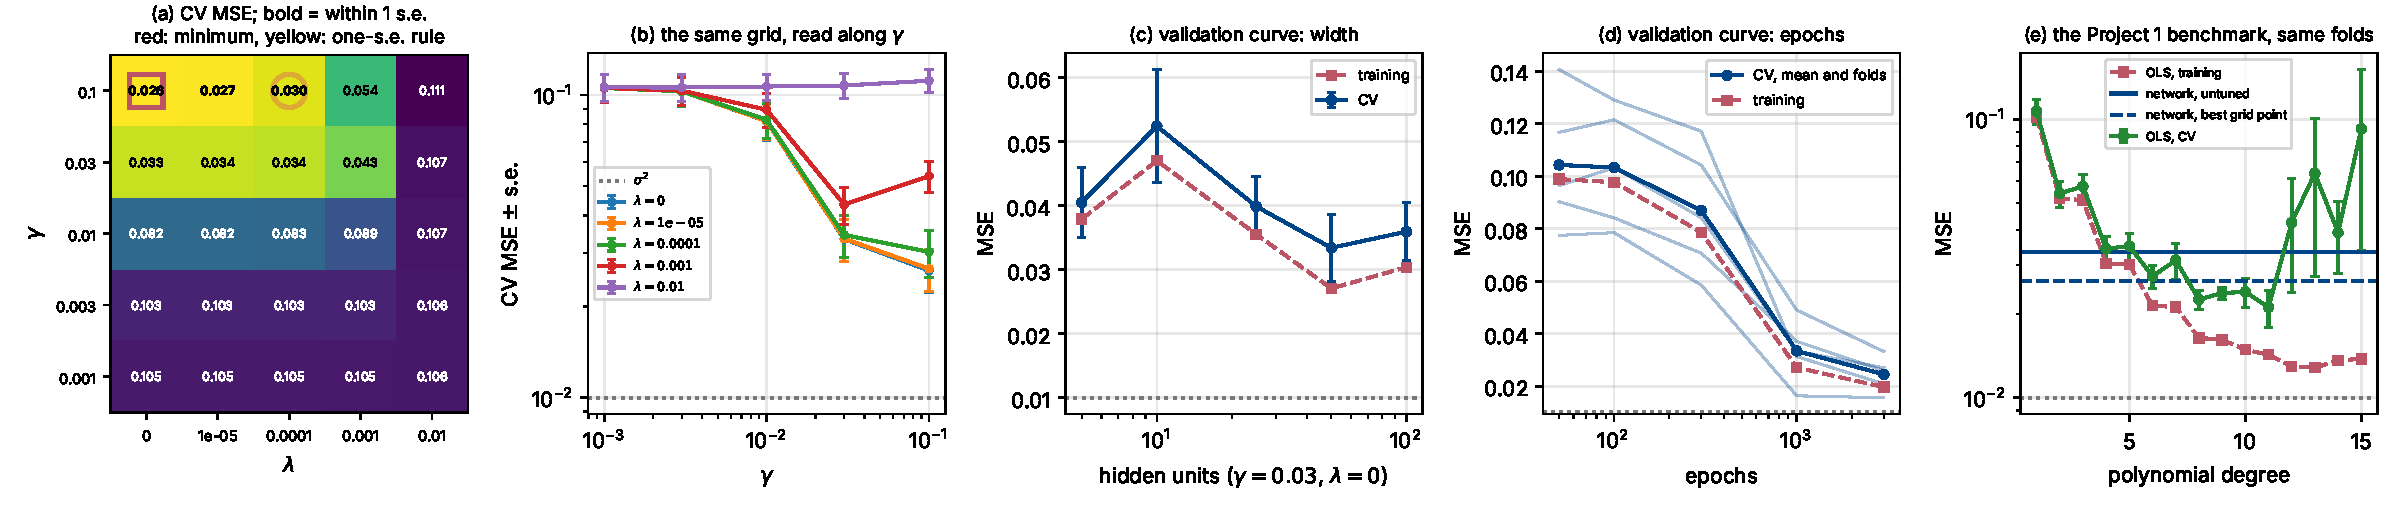
\includegraphics[width=0.99\textwidth]{week44_cv}
\end{center}
\small
(a) The $5\times5$ grid; bold cells are within one standard error of the
minimum (red); the one-standard-error choice (yellow) is the largest
$\lambda$ among them.  (b) The same numbers read along $\gamma$.  (c)--(d)
Validation curves over width and epochs with the training curves beside
them (the optional step 4).  (e) OLS polynomials on the same folds against
the network before and after the grid.
\end{frame}

\begin{frame}{Case 2: the numbers behind the figure (steps 2--4)}
\small
\begin{block}{Step 2: the untuned $1$--$50$--$1$ network}
Folds $0.031,\ 0.049,\ 0.016,\ 0.033,\ 0.037$; CV MSE $0.0334\pm0.0053$,
training $0.0271$.  Above $\sigma^{2}=0.01$, and the folds differ by a
factor of three -- why one number without an error bar means little.
\end{block}
\begin{block}{Step 3: the grid}
Minimum at $\gamma=0.1$, $\lambda=0$: $0.0263\pm0.0041$; three cells
within one standard error; the one-SE rule picks $\gamma=0.1$,
$\lambda=10^{-4}$ ($0.0303$) -- a weak preference, since $\lambda\le10^{-4}$
changes nothing the data can see.  The learning rate matters most: at
$\gamma=0.001$ the network has not converged in $1000$ epochs ($0.105$,
the variance of $y$), at $\gamma=0.1$ it has.  The penalty does nothing
until $10^{-2}$, where it hurts.
\end{block}
\begin{block}{Step 4: the curves}
Width: CV MSE $0.041,0.052,0.040,0.033,0.036$ for $5,10,25,50,100$ units
with standard errors $0.005$--$0.009$: no trend the error bars resolve --
at this $\gamma$ and $1000$ epochs the width is not what limits the fit.
Epochs: $0.104,0.103,0.087,0.033,0.025$ for $50,\dots,3000$ -- still
falling at $3000$ with $\gamma=0.03$: under-trained, not over-trained;
early stopping would not stop it yet.
\end{block}
\end{frame}

\begin{frame}{Case 2: the numbers behind the figure (steps 5--6)}
\small
\begin{block}{Step 5: the benchmark}
OLS: degree $11$, CV MSE $0.0211\pm0.0032$; Ridge: degree $11$,
$\lambda=10^{-4}$, $0.0210$.  The untuned network ($0.033$) is worse than
the polynomial; the tuned one ($0.026$) is within one standard error of
it -- with $151$ parameters against $12$ and $0.6$ s per fit against
milliseconds.
\end{block}
\begin{block}{Step 6: the test set, once}
Network \texttt{best\_estimator\_}: $0.0148$; OLS: $0.0133$; Ridge:
$0.0135$.  All three are \emph{below} their CV scores ($0.026$, $0.021$)
-- the opposite of what the optimism of Part A.14 predicts.  Two effects
compete: the refit on $100$ points instead of $80$ (more data, and $25\%$
more SGD steps per epoch) pulls the error down; the selection of the
minimum pushes the CV score down.  Here the first wins; on another test
draw it might not.  One test number has no error bar either.
\end{block}
\begin{block}{What goes into Project 2}
The $(\gamma,\lambda)$ heat map with the one-SE cell marked, the benchmark
table, \emph{one} test number per model, and a sentence on how each
hyperparameter was chosen.  The validation curves over width and epochs
only if you did the optional step 4.
\end{block}
\end{frame}

\begin{frame}{Case 2: do you have the insight?}
\small
\begin{enumerate}
  \item \texttt{GridSearchCV} refits the best point on all $100$ points.
        Why is the CV error of that point \emph{not} the error you should
        expect from \texttt{best\_estimator\_} -- in which direction is it
        off, and for two different reasons?
  \item The validation curve over epochs is still falling at $3000$.  Does
        that mean more epochs are always better for this network?  What
        would you do before concluding?
  \item The polynomial of degree $11$ and the tuned network are within one
        standard error of each other.  Which do you report as ``better'' in
        Project 2, and what sentence goes with the number?
  \item Someone runs the grid with \texttt{cv=KFold(5)} without
        \texttt{shuffle=True}.  The data cell sorted $x$.  What goes wrong?
\end{enumerate}
\pause
\begin{block}{What we hope you say}
\footnotesize
(1) The CV score is pessimistic because the fold models had $80$ points
instead of $100$, and optimistic because it is the minimum of $25$ noisy
estimates; which wins depends on the problem -- here the test MSE came out
\emph{below} the CV score, so the first did.  (2) No: at $\gamma=0.03$ the
optimiser is slow and the curve says ``not converged''; raise $\gamma$ (the
grid did) or add momentum, then look again -- a validation curve over
epochs is a statement about \emph{this} optimiser at \emph{this} learning
rate.  (3) Neither: report both with their error bars and say they cannot
be told apart on $100$ points; prefer the polynomial on simplicity and
speed unless the network wins elsewhere.  (4) The folds are contiguous
intervals of $x$: every fold model extrapolates to a region it never saw,
the CV error is pessimistic and the chosen hyperparameters are the ones
that extrapolate least badly, not the ones that fit best.  Shuffle.
\end{block}
\end{frame}

%% =====================================================================
\begin{frame}[fragile]{Only a mention: the same with PyTorch and Keras}
\small
\begin{block}{Nothing changes in the theory, and \texttt{KFold} only makes indices}
\begin{lstlisting}
for train_idx, val_idx in KFold(5, shuffle=True, random_state=2026).split(X):
    scaler = StandardScaler().fit(X[train_idx])        # inside the fold
    net = build_torch_model()                          # a fresh model
    train(net, scaler.transform(X[train_idx]), y[train_idx])
    errors.append(mse(net, scaler.transform(X[val_idx]), y[val_idx]))
\end{lstlisting}
Ten lines around any training function, the Monday CNN included; the
discipline -- scaler inside, fresh model per fold, test set once -- is
yours to keep, since nothing enforces it.
\end{block}
\begin{block}{Or make the framework model a \texttt{scikit-learn} estimator}
\texttt{skorch.NeuralNetRegressor} wraps a PyTorch module,
\texttt{scikeras.wrappers.KerasRegressor} a Keras model; both obey the
three rules, so \texttt{GridSearchCV} and \texttt{Pipeline} work as in
Case 2.
\end{block}
\begin{block}{Built-in validation, which is a single split}
Keras: \texttt{model.fit(X, y, validation\_split=0.2,
callbacks=[EarlyStopping(patience=10, restore\_best\_weights=True)])};
PyTorch: \texttt{random\_split} and the loop by hand.  Cheaper than $k$
folds, no standard error; the warnings carry over (the split is the
\emph{last} fraction, unshuffled; scale inside it; the test set is still
touched once).  None of this is needed for Project 2.
\end{block}
\end{frame}

\begin{frame}{Wrap-up, the exercises, and next week}
\footnotesize
\begin{block}{Before Friday (exercises week 44, deadline October 30)}
Exercise 1: the six questions, written out.  Exercise 2: Case 2 on your own
network -- the wrapper, the $(\gamma,\lambda)$ grid with the heat map and
the one-SE cell, the benchmark on the same folds, the test set once; the
validation curves over width and epochs (2c--d) are optional.
Exercise 3 (optional): the MNIST classifier with \texttt{StratifiedKFold},
\texttt{cross\_val\_predict} and the out-of-fold confusion matrix.
Exercise 4 (optional): the loop written by hand, checked against the
library -- the solution is in the notebook.  Declare your use of LLMs.
\end{block}
\begin{block}{Project 2 (deadline November 6)}
Required: $\gamma$ and $\lambda$ (L2/L1) chosen by cross-validation --
today's heat map and table; cross-validating depth, nodes, activation and
epochs is optional.  Part e) is the confusion matrix of week 43.  Every test
number comes from a model whose choices were made on training data alone --
say how.
\end{block}
\begin{block}{Three sentences to take home}
The training error chooses nothing.  The cross-validation error chooses
the hyperparameters and comes with an error bar that is too small.  The
test error is computed once and chooses nothing either.
\end{block}
\begin{block}{Next Monday, week 45}
Chapter 11, recurrent neural networks, and time for your Project 2
questions.  Reading for today: Sections 2.12, 3.14, 8.12; the
\texttt{scikit-learn} user guide (cross-validation, developing estimators).
\end{block}
\end{frame}

\end{document}
